\section{Implementierung}
\label{sec:model-implementation}

Dieser Abschnitt beschreibt die Implementierung des Modells.
Für den Aufbau und das Training werden TensorFlow 2.0\footnote{https://www.tensorflow.org/beta} sowie das mittlerweile darin integrierte Framework Keras\footnote{https://keras.io/} verwendet.
Die Implementierung kann grundsätzlich in drei Komponenten aufteilt werden:

\paragraph{Loader} Der Loader übernimmt die Aufgabe, die Trainings-Daten bereitszustellen.
Das Training des Modells wird im sog. Mini-Batch-Verfahren vollführt.
Der Loader lädt damit mit einem Python-Generator für jede Trainingsepoche nacheinander mehrere Ausschnitte des Gesamtdatensatzes (siehe Listing \ref{lst:mini-batch-loader}).
Dies ermöglicht, beliebig grosse Datensätze zu bearbeiten, da immer nur der Speicherbedarf eines Mini-Batches benötigt wird.

\begin{lstlisting}[language=Python, caption=Mini-Batch Loader, label=lst:mini-batch-loader]
    ...
    # Load mini-batch
    for dataframe in read_csv(
        filepath_or_buffer='data.csv',
        delimiter=',',
        header=0,
        chunksize=1000):

        # Iterate over lines in mini-batch
        for row in dataframe[dataframe.columns[1]]:
            ...
\end{lstlisting}

Der Loader übernimmt zudem die Aufgabe, die einzelnen Textsequenzen in einzelne Trainingseinheiten zu zerlegen.
Die Sequenzlänge für das Training des RNN's ist konstant.
Ist eine Trainingssequenz kürzer als die Fenstergrösse, wird sie mit Platzhalter Zeichen aufgefüllt («padding»).
Ist eine Trainingssequenz länger als die Fenstergrösse, so wird sie abgeschnitten.
Eine Trainingssequenz wird so Buchstabe um Buchstabe durch das Fenster geschoben.
Der letzte Buchstabe wird jeweils als Zielwert abgeschnitten und in einem separaten Array zurückgeliefert (y).
Gleichzeitig werden die Buchstabensequenzen mit dem Tokenizer in Vokabular-Indizes umgewandelt.
Zuletzt werden diese Vokabularfolgen in One-Hot-Vektoren umgewandelt.

\begin{lstlisting}[language=Python, caption=Encoding, label=lst:one-hot-encoding]
    windowed_tokenized_sequences = []

    # Split menu text up into characters
    split_text = list(row)
    split_text_with_end = split_text + ['<end>']

    # Generate windows
    for window_end in range(0, len(split_text_with_end)):

    padding_length = char_window_size - window_end

    windowed_tokenized_sequences.append([
    tokenizer.word_index.get(char, tokenizer.word_index.get('pre')) for char in (
    ['pad'] * max(0, padding_length) + split_text_with_end[max(0, window_end-char_window_size):window_end + 1])
    ])

    # print(windowed_tokenized_sequences)

    windowed_tokenized_sequences = np.array(windowed_tokenized_sequences)
    # print(tokenizer.sequences_to_texts(windowed_tokenized_sequences[:, :-1]))
    # print(tokenizer.sequences_to_texts([windowed_tokenized_sequences[:, -1]]))
    tokenized_char_phrases_X, tokenized_chars_y = windowed_tokenized_sequences[:, :-1], windowed_tokenized_sequences[:, -1]
    padded_phrases_X = pad_sequences(tokenized_char_phrases_X, char_window_size)

    one_hot_phrases = to_categorical(padded_phrases_X, num_classes=len(tokenizer.index_word) + 1)
    # print(padded_phrases_X)
    # print(one_hot_phrases)
    one_hot_ys = to_categorical(tokenized_chars_y, num_classes=len(tokenizer.index_word) + 1)
\end{lstlisting}


\paragraph{Builder} Die Builder-Komponente übernimmt die Aufgabe, das RNN-Modell nach bestimmten Vorgaben aufzubauen.
Sie scant durch sämtliche Datensätze und nimmt alle vorkommenden Buchstaben (=Vokabular) in einem sog. «\glq{Tokenizer}» auf.

\paragraph{Tainer} Trainer ist die Hauptkomponente, die vom Loader und vom Builder gebrauch macht.

\subsection{Evaluierung der schnellsten Batchsize}
\label{sec:evaluating-fastest-batchsize}
Während der ersten Versuche konnte eine unterschiedliche Ausführungsgeschwindigkeit in Abhängigkeit der Batch-Grösse beobachtet werden.
Um das Training der verschiedenen Modellkonfigurationen möglichst effizient

Grafikkarte 980XT.
Um das Modell möglichst effizient zu trainieren, soll die effizienteste Batch-Grösse für diese Grafikkarte empirisch eruiert werden.
Dazu werden 10 Epochen mit jeweils 1000 Trainingsschritten vollführt.

\begin{center}
    \begin{table}
        \centering
        \begin{tabular}{ |l|l| }

            \hline
            \textbf{n} & \textbf{Batch-Grösse} & \textbf{Durchschnittliche Dauer in Sekunden (über 10 Epochen)} \\
            \hline
            1 & 14.69 \\
            50 & 4.07 \\
            71 & 4.04 \\
            91 & 3.97 \\
            100 & 3.93 \\
            125 & 3.98 \\
            200 & 5.32 \\
            250 & 6.16 \\
            \hline
        \end{tabular}
        \caption{Altes Modell}
        \label{tab:best-batch-size}
    \end{table}
\end{center}

\begin{center}
    \begin{table}
        \centering
        \begin{tabular}{ |l|l| }

            \hline
            \textbf{n} & \textbf{Batch-Grösse} & \textbf{Durchschnittliche Dauer in Sekunden (über 10 Epochen)} \\
            \hline
            1 & 55.52 \\
            2 & 53.14 \\
            10 & 49.82 \\
            25 & 15.86 \\
            50 & 1.74 \\
            71 & 1.69 \\
            91 & 1.67 \\
            100 & 1.67 \\
            125 & 1.73 \\
            143 & 1.77 \\
            200 & 2.15 \\
            250 & 2.44 \\
            \hline
        \end{tabular}
        \caption{Neues Modell}
        \label{tab:best-batch-size-new}
    \end{table}
\end{center}

\subsection{Erweiterung des Trainingssets}
\label{subsec:enhancing-training-set}

-- INSERT HISTORGRAM LINE LENGHTS ---

Bisher war das Modell so implementiert, dass jede Epoche jeweils die gleichen Trainingseinheiten erhielt.
Der Grund für dieses Vorgehen basierte auf der Annahme, dass jede Trainingseinheit mehrmals dem Modell vorgelegt werden müsse, damit
ein der Lernprozess effektiv ist.
Diese Annahme entstand jedoch auf der fehlerhaften Implementierung, weshalb sie verworfen werden kann.
Der Nachteil dieses Vorgehens bestand darin, dass das Modell eine relativ begrenztes Trainingsset zu sehen bekam.
Dieser Nachteil verstärkt sich, da durch das behobene und nun korrekt funktionierende Training noch weniger Trainingseinheiten verwendet werden.
Bei einer Median-Zeilenlänge von 26 Zeichen, 500 Batches à 100 Trainingsschritten werden dem Modell also:

\[ 500 \cdot \frac{100}{26} = 1'923.1 \]

gerade mal rund 1900 Zeilen der insgesamt 400'000 Zeilen gezeigt.
Damit erlernt das Modell ein sehr begrenztes Vokabular.
Die Trainingslogik soll nun so verbessert werden, dass jede Epoche einen beliebigen Ausschnitt aus allen Zeilen zum Training erhält.
Der Loader wird als endloser Generator implementiert.
Erreicht eine Epoche das Ende des Datensatzes, wird einfach wieder von vorne begonnen.
Gleichwohl mit dem Datensatz, der zur Validierung herangezogen wird.
Der Generator wird also quasi als Ringspeicher implementiert wobei Trainings- und Validierungsdatensatz um die Hälfte der Länge des Gesamtdatensatzes
verschoben («Offset») ausgeliefert werden.
Damit das ganze Datenset mindestens einmal durchlaufen wird müssten also insgesamt rund \[ 26 \cdot 422039 = 10'973'014 \] Trainingsschritte vollführt werden.
Wird von einer idealen Batchsize von 100 Trainingsschritten ausgegangen, fallen insgesamt \[ \frac{10973014}{100} = 109'730 \] Batches an.
Damit kann die Anzahl der notwendigen Batches für eine bestimmten Prozentsatz des Gesamtdatensatzes als Funktion $ b(p, e) $ ausgedrückt werden:

\[ b(p, e) = \frac{p \cdot R \cdot S}{B * e} \]

wobei $ p $ dem gewünschten Anteil entspricht, $ e $ die Anzahl Epochen darstellt und die Konstanten $ R $, $ S $ sowie $ B $ die Anzahl Trainingssätze (Zeilen), die durchschnittliche Zeichenzahl pro Zeile sowie
die ideale Batch-Grösse repräsentieren.

Sollen also beispielsweise 25\% des gesamten Datensatzes mit 50 Epochen trainiert werden, so fallen:

\[ b(0.25, 50) = \frac{0.25 \cdot 422039 \cdot 26}{125 \cdot 50} = 438.92 \]

Batches an.

\subsection{Hinzufügen der Zeitkomponente}
\label{subsec:adding-time-component}

Jeder Trainingssatz bzw. jede Gerichtbezeichnung ist mit einem Datum versehen, an dem das Gericht zum ersten Mal
registriert wurde sowie mit einem Datum, an dem das Gericht zum letzen Mal registriert wurde.
Ein Histogram legt offen, dass die einzelnen Gerichte ungleichmässig auf die Zeit verteilt ist.
Ausserdem weist der Grossteil der Gerichte eine «Lebensdauer» von wenigen Jahren auf (siehe Abb.\ref{fig:hist-dates-datespans}).
Aufgrund letztgenannter Tatsache soll das Enddatum einfachheitshalber ignoriert werden.
Stattdessen wir das Eintrittsdatum der Eingabesequenz für das Modell angehängt.
Da nach erstem Ausprobieren das Anfügen der absoluten Jahreszahl kein gutes Training ermöglichte, wird das Jahr
als relativer Wert in einer Jahresspanne von 300 Jahren (1800 - 2100) angehängt, wobei also 0.0 dem Jahr 1800 sowie
der Wert 1.0 dem Jahr 2100 entsprechen.

\begin{figure}
    \centering
    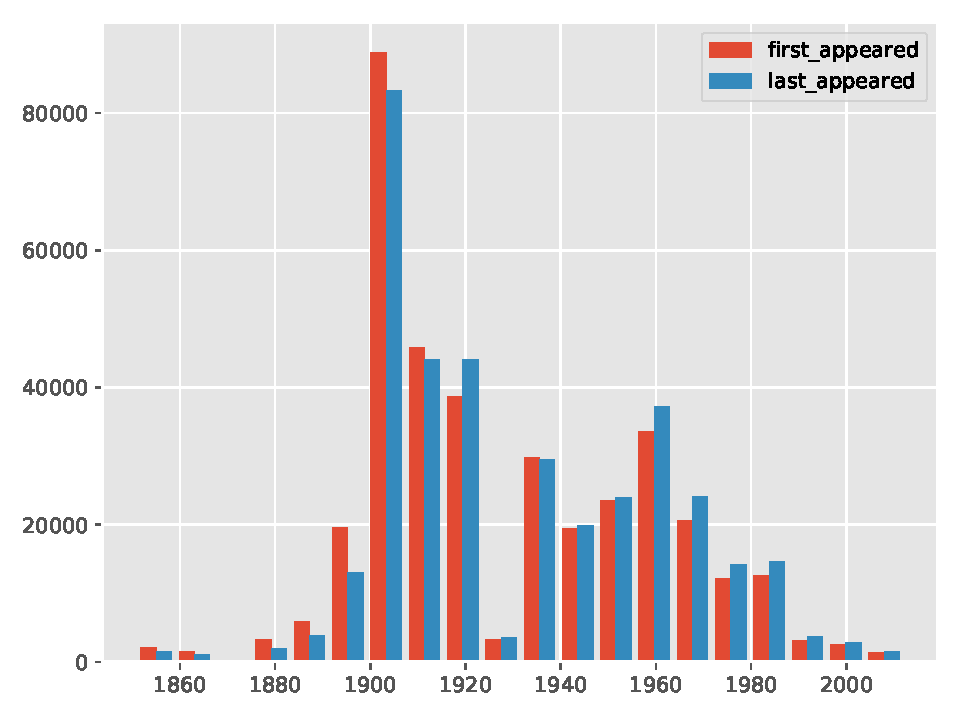
\includegraphics[width=0.75\linewidth]{images/analysis/histogram-dates.pdf}
    \caption{Zeitliche Verteilung}
    \label{fig:hist-dates-datespans}
\end{figure}

Dem Modell werden zudem sog. Callbacks\footnote{https://keras.io/callbacks/} hinzugefügt, damit das Training nach
längerem Plateau nicht unnötig weiter trainiert werden muss.
Ausserdem wird das gesamte Modell und insbesondere seine Gewichte nach jeder Epoche quasi als «Spielstand» gespeichert,
falls sich die Validierungsakuratheit insgesamt verbessert hat.
